\section{Introduction}
\label{sec:intro}

The rapid scaling of Large Language Models (LLMs) into the 100B-1T parameter regime has pushed the limits of modern training infrastructure. To mitigate the growing demands on memory and computation, Mixture-of-Experts (MoE) architectures have emerged as a dominant paradigm for efficient scaling~\cite{gshard2021, mixtral2024, deepseekv3, kimik22025, gptoss2025}, activating only a sparse subset of expert parameters per token and thus decoupling model capacity from per-token compute.

Alongside architectural innovations, low-precision formats such as FP8 and FP4 have gained increasing attention for their ability to reduce memory footprint and improve arithmetic throughput, particularly for bandwidth- and memory-bound workloads. Prior work has shown that carefully designed low-precision training can preserve convergence while significantly improving system efficiency~\cite{deepseekv3, mxfp8recipe}. Recent hardware advances—most notably NVIDIA's Blackwell GPUs—enable native FP4 tensor core support, allowing aggressive quantization with minimal impact on convergence~\cite{mxfp4training2025, nvfp4training2025}. However, such support is not yet available on the majority of current-generation accelerators—particularly Hopper GPUs—which lack both FP4 compute and communication primitives.

This hardware gap presents significant challenges for adopting FP4 in existing training pipelines, especially for MoE models where activation memory and expert-parallel communication dominate system cost. Deploying FP4 on Hopper-class GPUs without native support introduces multiple technical obstacles: quantized formats such as MXFP4 rely on block-wise power-of-two scaling incompatible with Hopper's FP8 pipeline; intermediate conversions (e.g., FP8 $\leftrightarrow$ BF16 $\leftrightarrow$ FP4) incur latency and memory overhead; and communication libraries must be redesigned to support sub-byte packing and efficient dequantization.

In this work, we address these challenges by proposing a hybrid-precision MXFP4 training framework that enables FP4-level memory and communication efficiency on Hopper GPUs. Our approach compresses activations and all-to-all dispatches into software-emulated MXFP4 format, while preserving FP8 precision in compute-intensive GEMM operations. This design decouples compute and storage precision, maintains compatibility with Transformer Engine and DeepEP, and avoids lossy intermediate conversions—ensuring both numerical stability and practical deployment efficiency.

\vspace{1mm}
\noindent \textbf{Our contributions are as follows:}
\begin{itemize}
    \item We introduce an FP4 communication and caching strategy for expert-parallel MoE layers, reducing activation memory and inter-GPU traffic by over 50\%.
    \item We design a direct bitwise FP4-to-FP8 conversion algorithm with hierarchical scale alignment, eliminating the need for BF16 intermediates.
    \item We implement layout-aware CUDA kernels optimized for quantization, dispatch, and recomputation in FP4, including native support for ragged MoE tensors and transposed data layouts.
    \item We present the first production-scale deployment of software-emulated MXFP4 for MoE training on Hopper GPUs. At the 671B parameter scale, our method reduces peak activation memory by 14.8\% (11.8 GB), improves throughput by 12.5\% (from 1157 to 1302 tokens/GPU/s), and matches the convergence of strong FP8 baselines.
\end{itemize}

We release our full training implementation (Appendix~\ref{sec:appendix-code}) to facilitate reproducibility and adoption. Figure~\ref{fig:overview} provides a high-level overview of our approach.

\begin{figure}[htb]
    \centering
    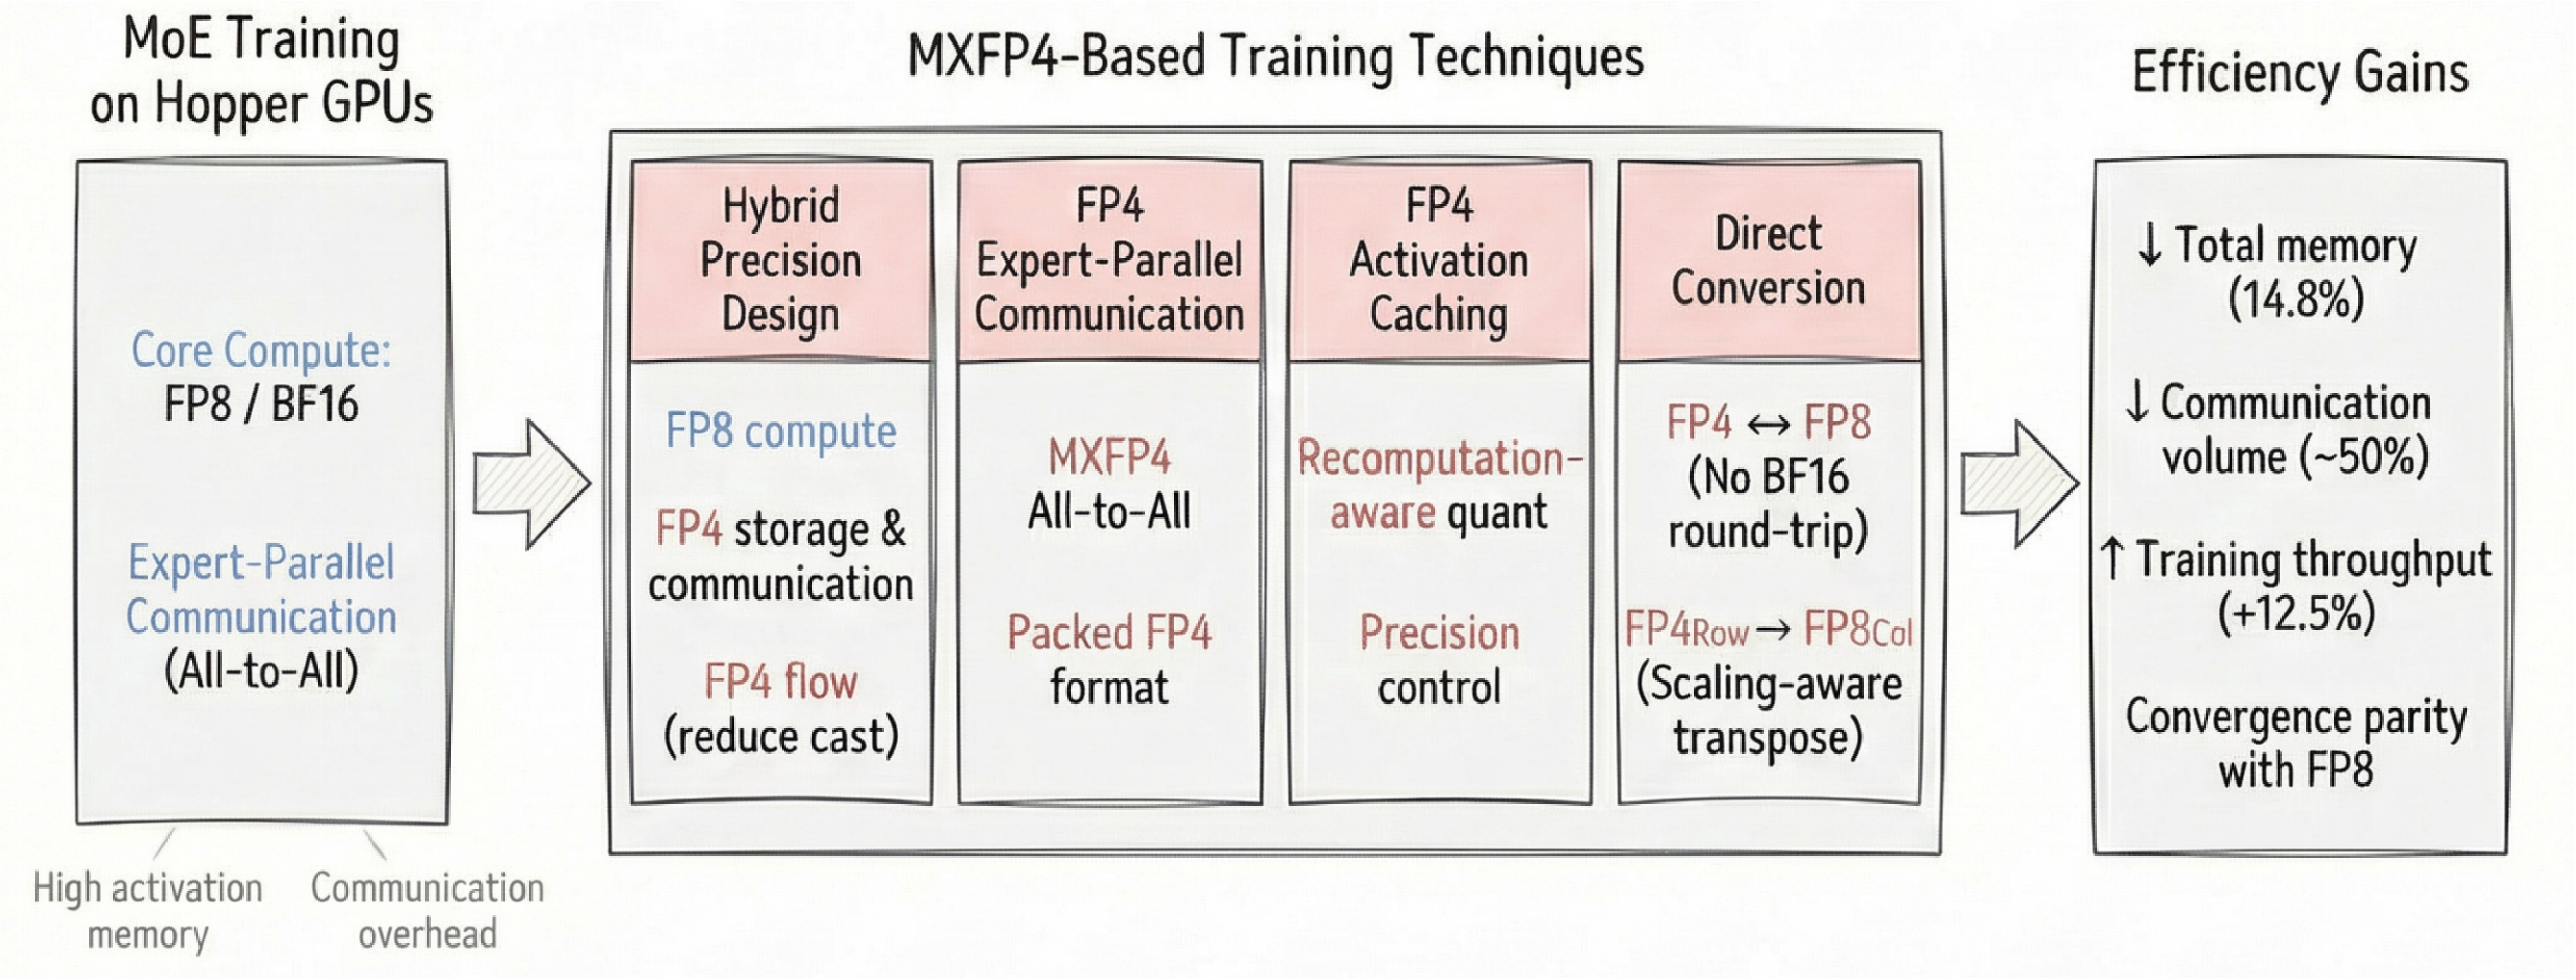
\includegraphics[width=\linewidth]{images/fp4overview_opt.pdf}
    \caption{MXFP4-based MoE training on Hopper GPUs.}
    \label{fig:overview}
\end{figure}
